%<dscrpt>Méthodes de Picard et d'Euler, lemme de Gronwall. </dscrpt>
On se propose de démontrer l'existence et l'unicité puis d'approcher numériquement une fonction $y$ définie continue dérivable dans $[0,1]$ et vérifiant :
\begin{displaymath}
\left\lbrace \begin{aligned}
 & y(0) = 0 \\
 & \forall t\in [0,1] : y'(t) = \frac{1}{2}\left( t^2 + y^2(t)\right) 
\end{aligned}
\right. 
\end{displaymath}
\subsection*{I. Existence : méthode de Picard}
\begin{figure}[ht]
 \centering
 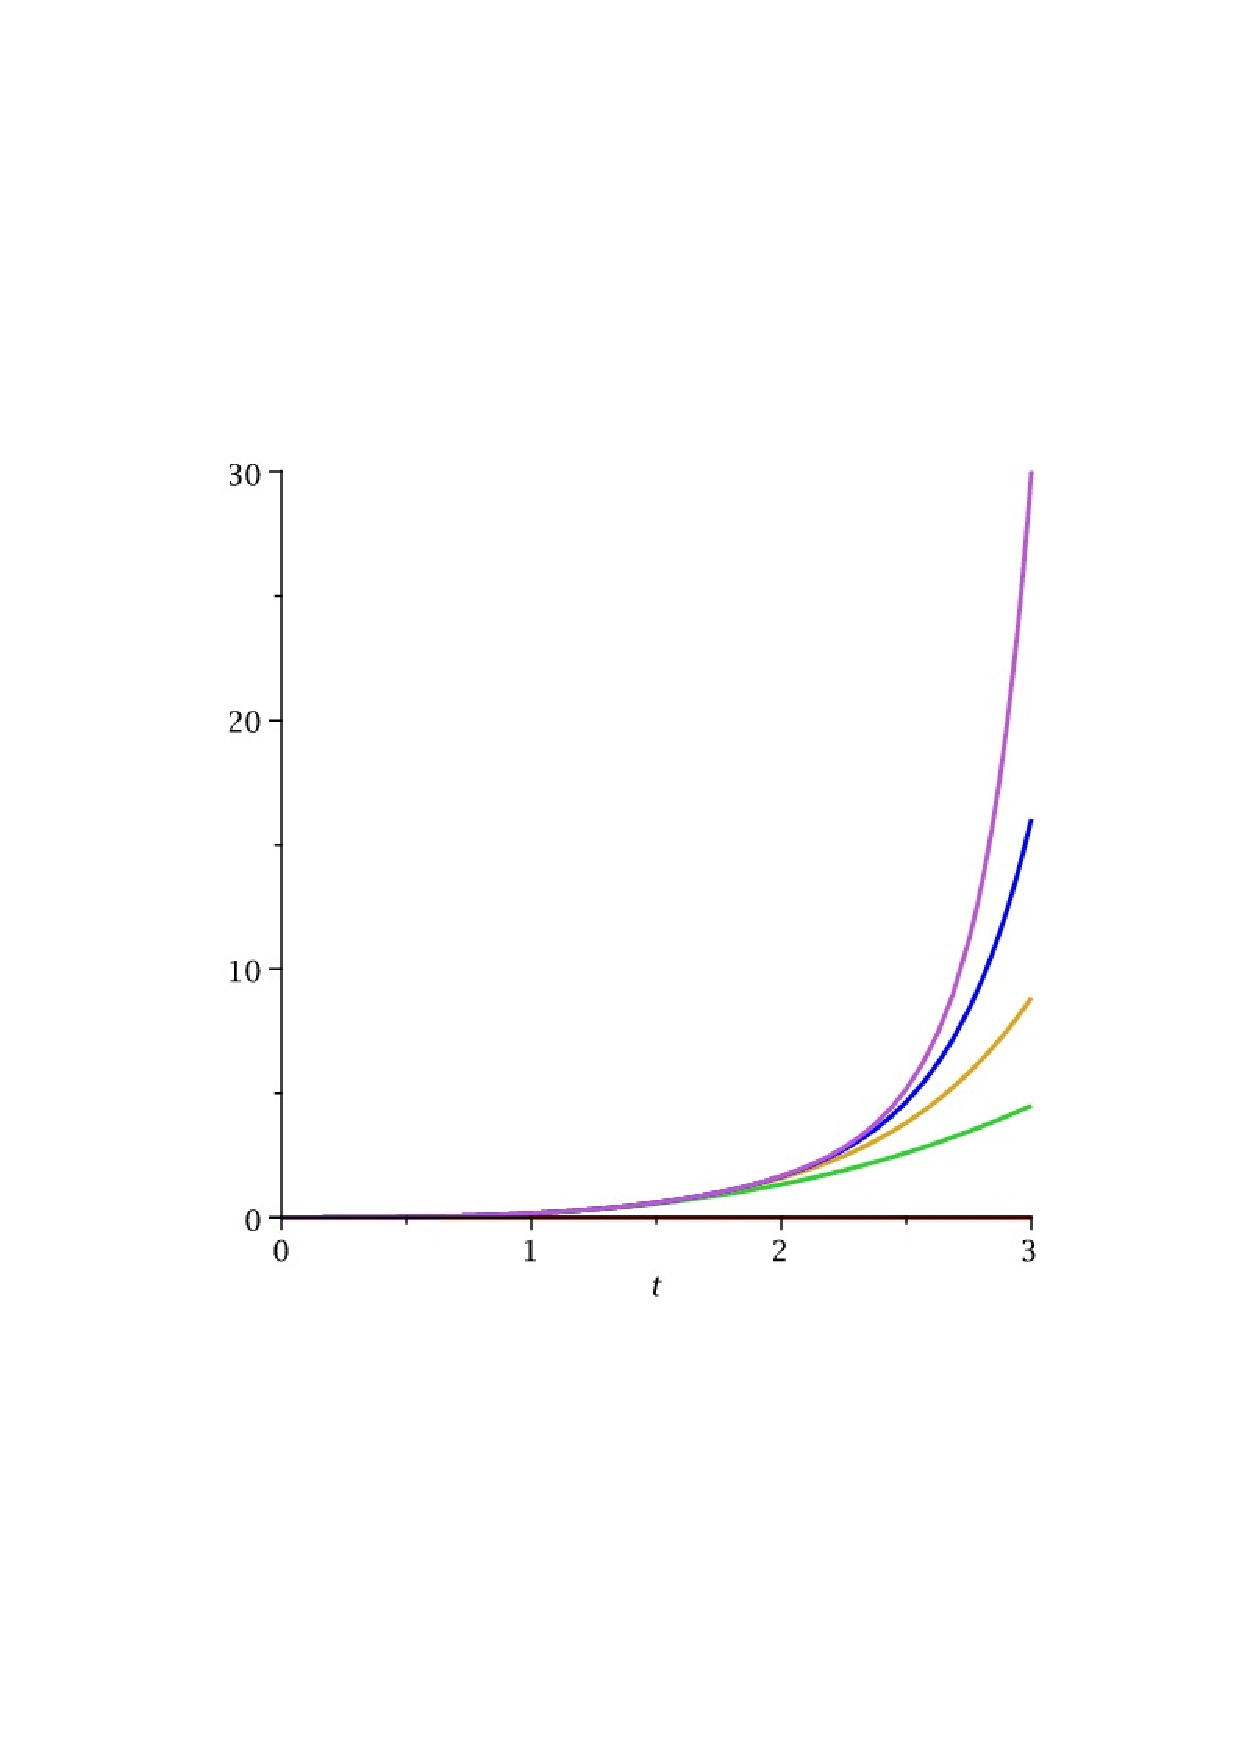
\includegraphics[width=8cm]{Eapprox1_1.pdf}
 % Eapprox1_1.png: 555x555 pixel, 72dpi, 19.58x19.58 cm, bb=0 0 555 555
 \caption{Portions de graphe de $y_0$, $y_1$, $y_2$, $y_3$, $y_4$}
 \label{fig:Eapprox1_1}
\end{figure}

Pour tout entier $n$, on définit une fonction polynomiale $y_n$ par les relations suivantes :
\begin{displaymath}
 \left\lbrace 
\begin{aligned}
&\forall t \in \R : y_0(t) = 0 \\ 
&\forall n\in \N , \forall t\in \R : y_{n+1}(t) = \frac{1}{2}\int_0^t\left(\tau^2 + y_n^2(\tau)\right)d\tau 
\end{aligned}
\right. 
\end{displaymath}
\begin{enumerate}
 \item \begin{enumerate}
 \item Calculer $y_1(t)$ pour tout réel $t$. 
\item Pour tout entier $n$, montrer que $y_n(0)=0$  et que la fonction $y_n$ est croissante. 
\item Montrer que 
\begin{displaymath}
 \forall n\in \N , \forall t\in [0,1] : 0\leq y_n(t) \leq 1
\end{displaymath}
\end{enumerate}

\item \begin{enumerate}
 \item Pour tout $t\in[0,1]$, montrer que la suite $\left(y_n(t) \right)_{n\in\N}$ est croissante. En déduire que cette suite est convergente. On note $y(t)$ la limite de cette suite.\newline
Ceci définit une fonction $y$ dans $[0,1]$. La notation $y$ désigne cette fonction \emph{dans toute la suite du problème}.
\item Montrer que $y(0)=0$ et que 
\begin{displaymath}
 \forall t\in [0,1] : 0\leq y(t) \leq 1
\end{displaymath}
\item Montrer que $y$ est lipschitzienne de rapport $1$ donc continue.
\end{enumerate}

\item Dans cette question $0<a<1$.
\begin{enumerate}
 \item Montrer que :
\begin{displaymath}
 \forall n \in \N, \forall t \in [0,a] : 0\leq y_{n+1}(t) - y_n(t) \leq a^n
\end{displaymath}
\item Montrer que :
\begin{displaymath}
 \forall n \in \N, \forall t \in [0,a] : 0\leq y(t) - y_n(t) \leq \frac{a^n}{1-a}
\end{displaymath}
\item Montrer que :
\begin{displaymath}
 \forall n \in \N, \forall t \in [0,a] :
 0\leq \frac{1}{2}\int_0^t\left(\tau^2+y^2(\tau) \right)d\tau  - y_{n+1}(t) \leq \frac{a^nt}{1-a}
\end{displaymath}
\end{enumerate}
\item \begin{enumerate}
 \item Montrer que 
\begin{displaymath}
 \forall t\in [0,1[ : y(t) = \frac{1}{2}\int_0^t\left(\tau^2+y^2(\tau) \right)d\tau
\end{displaymath}
\item Montrer que la formule précédente est valable aussi en $1$. En déduire que $y$ est une solution de l'équation différentielle donnée au début de l'énoncé.
\end{enumerate}
\end{enumerate}

\subsection*{II. Unicité : lemme de Gronwall}
On suppose qu'il existe deux solutions $y$ et $z$ dans $[0,1]$ de l'équation différentielle donnée au début. On définit la fonction $u$ par :
\begin{displaymath}
 \forall t\in [0,1] : u(t) = |y(t) -z(t)|
\end{displaymath}
On pose aussi :
\begin{displaymath}
 M = \max_{[0,1]}\left( |y| + |z|\right)
\end{displaymath}
\begin{enumerate}
 \item \begin{enumerate}
 \item Justifier l'existence de $M$. Montrer que, pour tout $t\in [0,1]$ :
\begin{displaymath}
 u(t) \leq \frac{M}{2}\int_0^t u(\tau)d\tau
\end{displaymath}
\item Montrer que pour tout $\varepsilon>0$ et tout $t\in[0,1]$ :
\begin{displaymath}
\frac{\frac{M}{2}u(t)}{\varepsilon + \frac{M}{2}\int_0^t u(\tau)d\tau}
\leq \frac{M}{2}
\end{displaymath}
\end{enumerate}
\item \begin{enumerate}
 \item Montrer que pour tout $\varepsilon>0$ et tout $t\in[0,1]$ :
\begin{displaymath}
\frac{\varepsilon + \frac{M}{2}\int_0^t u(\tau)d\tau}{\varepsilon}
\leq e^{\frac{M}{2}t}
\end{displaymath}
\item En déduire (lemme de Gronwall) que pour tout $\varepsilon>0$ et tout $t\in[0,1]$ :
\begin{displaymath}
 u(t) \leq \varepsilon \,e^{\frac{M}{2}t}
\end{displaymath}
\end{enumerate}

\item Montrer que $y(t)=z(t)$ pour tout $t\in[0,1]$.
\end{enumerate}


\subsection*{III. Approximation : méthode d'Euler}
\begin{figure}[ht]
 \centering
 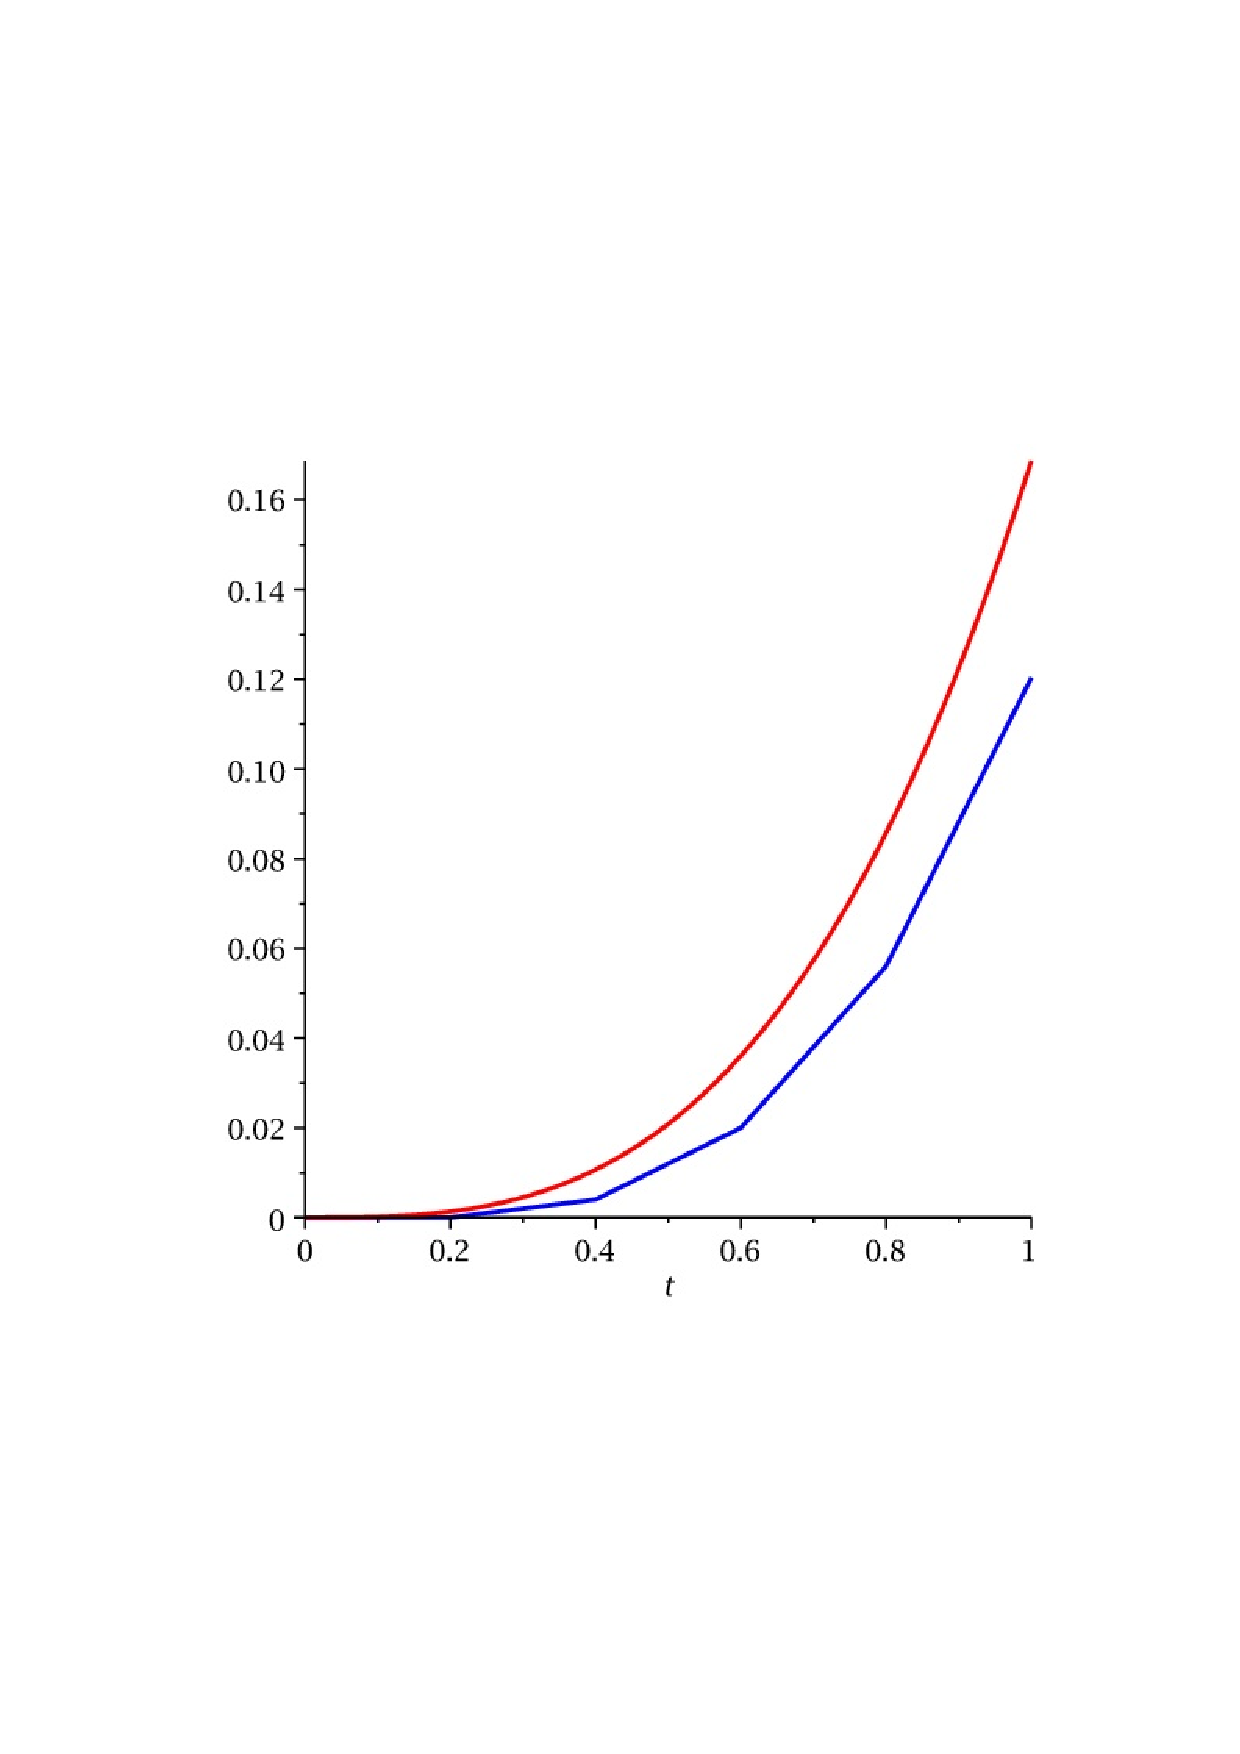
\includegraphics[width=8cm]{Eapprox1_2.pdf}
 % Eapprox1_2.png: 555x555 pixel, 72dpi, 19.58x19.58 cm, bb=0 0 555 555
 \caption{Méthode d'Euler pour $N=5$.}
 \label{fig:Eapprox1_2}
\end{figure}

Soit $N$ un entier naturel fixé, on pose $h = \frac{1}{N}$ et , pour tout entier $i$ entre $0$ et $N$, $t_i=ih$. On définit une famille de nombres réels $u_0,u_1,\cdots,u_N$ par :
\begin{displaymath}
 \left\lbrace 
\begin{aligned}
 & u_0 = 0 \\
&\forall i \in \{0,\cdots, N-1\} : u_{i+1} = u_i + \frac{h}{2}(t_i^2 + u_i^2)
\end{aligned}
\right. 
\end{displaymath}
Pour $i$ entre $1$ et $N$, on considère chaque $u_i$ comme une approximation de $y(t_i)$.\newline
 On pose $e_i=y(t_i)-u_i$ et on cherche à encadrer les $e_i$ c'est à dire à trouver une majoration de l'erreur.
\begin{enumerate}
 \item Montrer que pour tout réel $x\geq 0$ : $1+x \leq e^x$.
\item Soit $A$ et $B$ des réels strictement positifs, de plus $A\neq 1$. On considère deux suites $\left( e_n \right)_{n\in\N}$ et $\left( E_n \right)_{n\in\N}$ vérifiant :
\begin{displaymath}
 \begin{aligned}
&e_0 = 0 &,& &\forall n\in \N :  0\leq e_{n+1} &\leq Ae_n +B \\
&E_0 = 0 &,& &\forall n\in \N :  E_{n+1} &= AE_n +B 
 \end{aligned}
\end{displaymath}
\begin{enumerate}
 \item Montrer que $ e_n \leq E_n$ pour tous les entiers $n$.
 \item Montrer que pour tout entier $n$:
\begin{displaymath}
 e_n \leq \frac{B}{A-1}(A^n -1)
\end{displaymath}
\end{enumerate}

\item Soit $\varphi\in\mathcal C^1(|\alpha , \beta])$ et $M_1$ réel tel que $|\varphi'(t)|\leq M_1$ pour tous les $t\in [\alpha , \beta]$. Montrer que 
\begin{displaymath}
 \left \vert\int_\alpha ^\beta \varphi(t)dt - (\beta-\alpha)\varphi(\alpha)\right\vert
\leq \frac{M_1}{2}(\beta - \alpha)^2
\end{displaymath}

\item Pour tout entier $i$ entre $0$ et $N-1$, montrer que :
\begin{displaymath}
 e_{i+1} = e_i +\frac{1}{2}\int_{t_i}^{t_{i+1}}\left(t^2 - t_i^2 +y^2(t) - u_i^2 \right) dt
\end{displaymath}
\item \begin{enumerate}
 \item Pour tout entier $i$ entre $0$ et $N-1$, montrer que $0\leq e_i$ et que $0\leq u_i \leq 1$.
\item Pour tout entier $i$ entre $0$ et $N-1$, montrer que :
\begin{displaymath}
 e_{i+1} \leq (1+h)e_i + h^2
\end{displaymath}
\end{enumerate}

\item Pour tout entier $i$ entre $0$ et $N-1$, montrer que :
\begin{displaymath}
 e_i \leq h\left( (1+h)^N - 1\right) 
\end{displaymath}
En déduire
\begin{displaymath}
 0\leq e_i \leq h(e-1)
\end{displaymath}
\end{enumerate}
